\documentclass[12pt,letterpaper]{article}

\usepackage{amsmath, amsthm, amsfonts, amssymb}
\usepackage{microtype, parskip, graphicx}
\usepackage[comma,numbers,sort&compress]{natbib}
\usepackage{lineno}
\usepackage{longtable}
\usepackage{docmute}
\usepackage{caption, subcaption, multirow, morefloats, rotating}
\usepackage{wrapfig}
\usepackage{hyperref}

\frenchspacing

\begin{document}

\section{Results}

\subsection{Posterior predictive results}
% why do i want to show all these graphs?
%   demonstrate how well the model recapitulates the observed data
%   if the model simulates datasets like the one we observed
%     then we can be more confident in our inferences
%   PPCs by group reveal even more about the fit of our model
%     are some time bins better predicted by others?
%     well predicted time bins indicate congruence with model assumptions
%     poorly predicted time bins indicate incongruence with model assumptions
%       something different is happening in these bins that requires explanation



Overall, each taxonomic group is adequately described by the fitted model, where adequacy means that the posterior predictive distribution of our models resemble the empirical data it was fit to. 

A point comparison between the observed mean geologic unit diversities and the posterior predictive distributions for each taxonomic group indicate that our fitted models are able to recapitulate this aspect of the observed data (Fig. \ref{fig:ppc_mean}). This result is reassuring because our model is specifically a model of expected geologic unit diversity, and a good fit to mean diversity means our model fits are at least capturing this basic aspect of the data.

% overall ppc-s
% mean
\begin{figure}[ht]
  \centering
  
\includegraphics[width=\textwidth,height=0.5\textheight,keepaspectratio=true]{figure/ppc_mean}
  \caption{Posterior predictive results comparing the observed mean diversity of a geological unit for each of the studied taxonomic groups to a distribution of 1000 estimates from datasets simulated from the posterior predictive distribution of our models. Model adequacy is determined by how similar the posterior predictive distribution is to the observed value. In all cases, our models appear able to reproduce to observed means.}
  \label{fig:ppc_mean}
\end{figure}

Comparison of the observed standard deviation estimates for each of the taxonomic datasets to the posterior predictive distributions of our model fits show that our model is slightly over estimating the scale of our data, though not to a necessarily concerning degree (Fig. \ref{fig:ppc_sd}). Count data can frequently be over dispersed and have a standard deviation to mean ratio greater than 1; this reality is the reason we chose to use a truncated Negative-Binomial as opposed to a Poisson distribution because the addition of a second parameter allows us to model this overdispersion CITATIONS. While our model is not too different from the data, there is room for improvement in modeling the actual dispersion of geologic unit diversity.

% sd
\begin{figure}[ht]
  \centering
  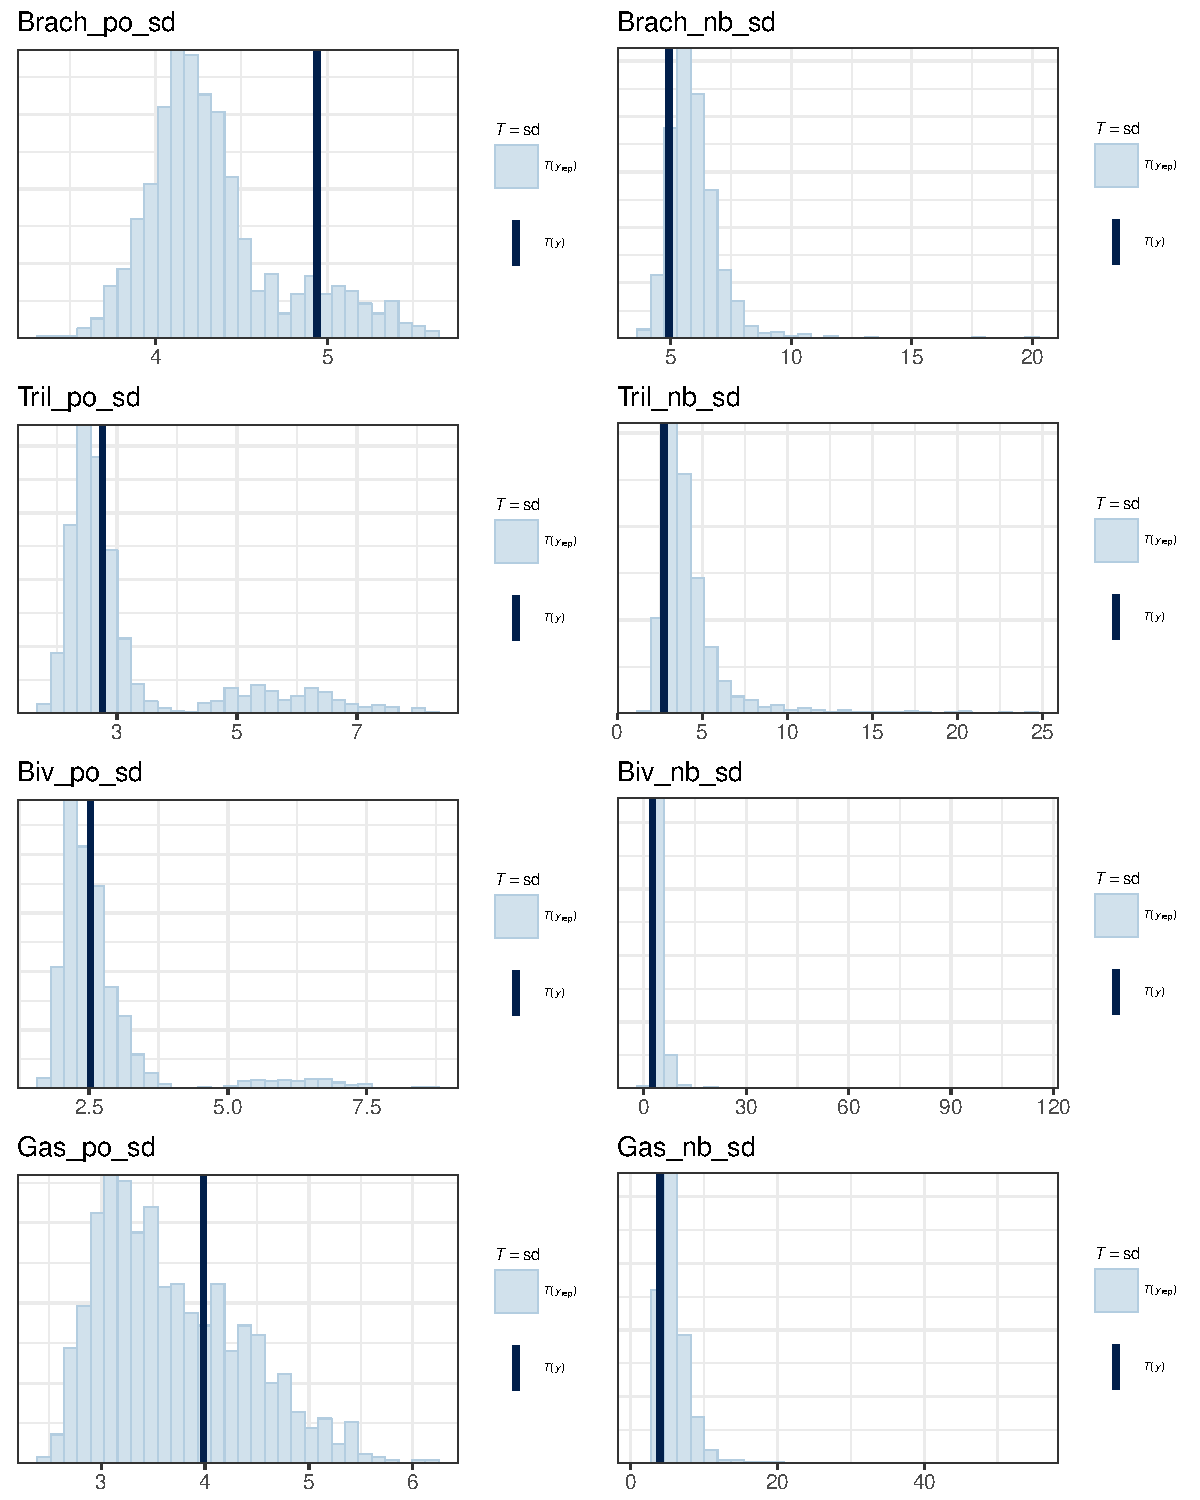
\includegraphics[width=\textwidth,height=0.5\textheight,keepaspectratio=true]{figure/ppc_sd}
  \caption{Posterior predictive results comparing the observed standard deviation diversity of a geological unit for each of the studied taxonomic groups to a distribution of 1000 estimates from datasets simulated from the posterior predictive distribution of our models. Model adequacy is determined by how similar the posterior predictive distribution is to the observed value. In all cases, our models appear able to reproduce to observed standard deviations.}
  \label{fig:ppc_sd}
\end{figure}


Comparisons of the empirical probability density functions for each of the taxonomic groups to the posterior predictive distribution of density functions generated by our model fits indicate that our model is very capable of recapitulating the observed data for nearly its entire range (Fig. \ref{fig:ppc_dens}). Importantly, the posterior predictive distributions have a heavier right tail than the empirical data; this means that the max estimated geologic unit diversity for some of our posterior predictive simulations is higher than the empirically observed maximum diversity. This observation helps illuminate the reason for the slight overestimate of the standard deviations of geologic unit diversity for the taxonomic groups (Fig. \ref{fig:ppc_sd}); our model is not as effectively estimating the right-tail of the observed distribution, an occurrence that is quite common as extreme values are by definition far away from the expected value which we are actually modeling CITATION. Additionally, the posterior predictive distributions of our models fit the data well in nearly all cases, indicating that our model is potentially capturing some aspects of the data generating process.

\begin{figure}[ht]
  \centering
  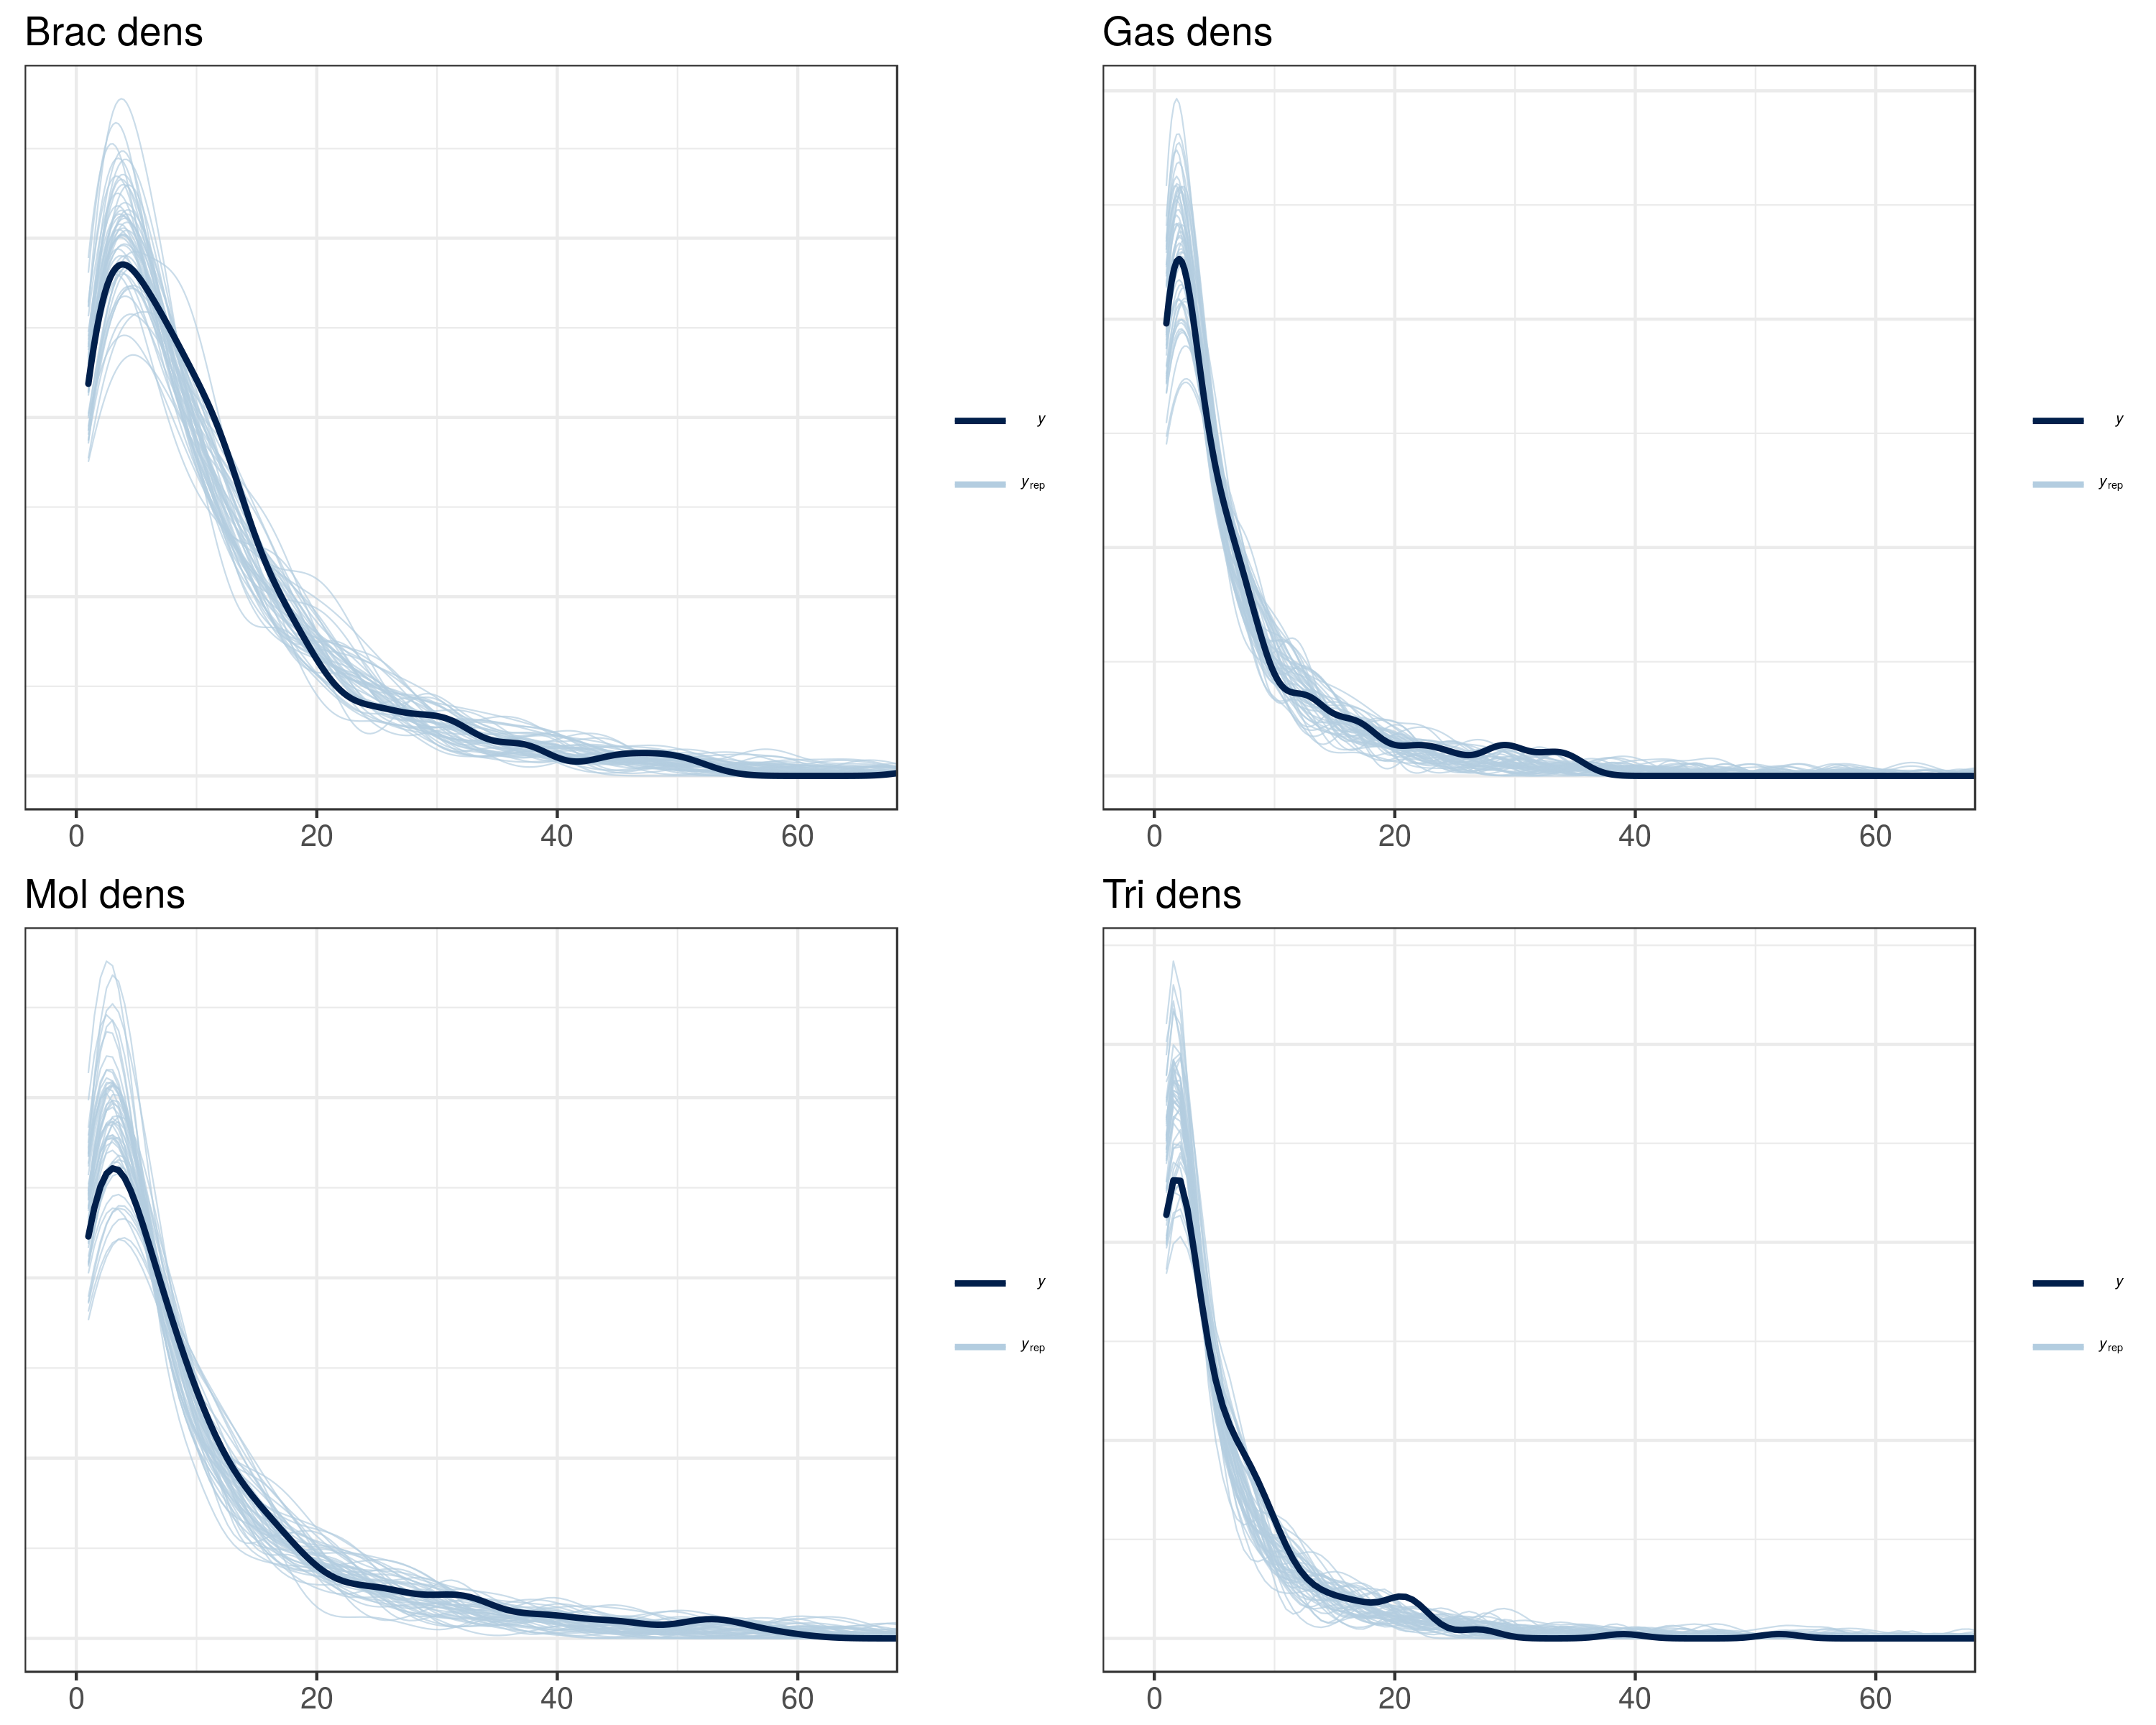
\includegraphics[width=\textwidth,height=0.5\textheight,keepaspectratio=true]{figure/ppc_dens_zoom}
  \caption{Posterior predictive results comparing the empirical probability density of a geological unit for each of the studied taxonomic groups to a distribution of 1000 probability densities from datasets simulated from the posterior predictive distribution of our models. Model adequacy is determined by how similar the posterior predictive distribution is to the observed value. In all cases, our models appear able to almost reproduce to observed ecdf-s.}
  \label{fig:ppc_dens}
\end{figure}

The cummulative distribution function is description of the normalized rank order accumulation of the data.

\begin{figure}[ht]
  \centering
  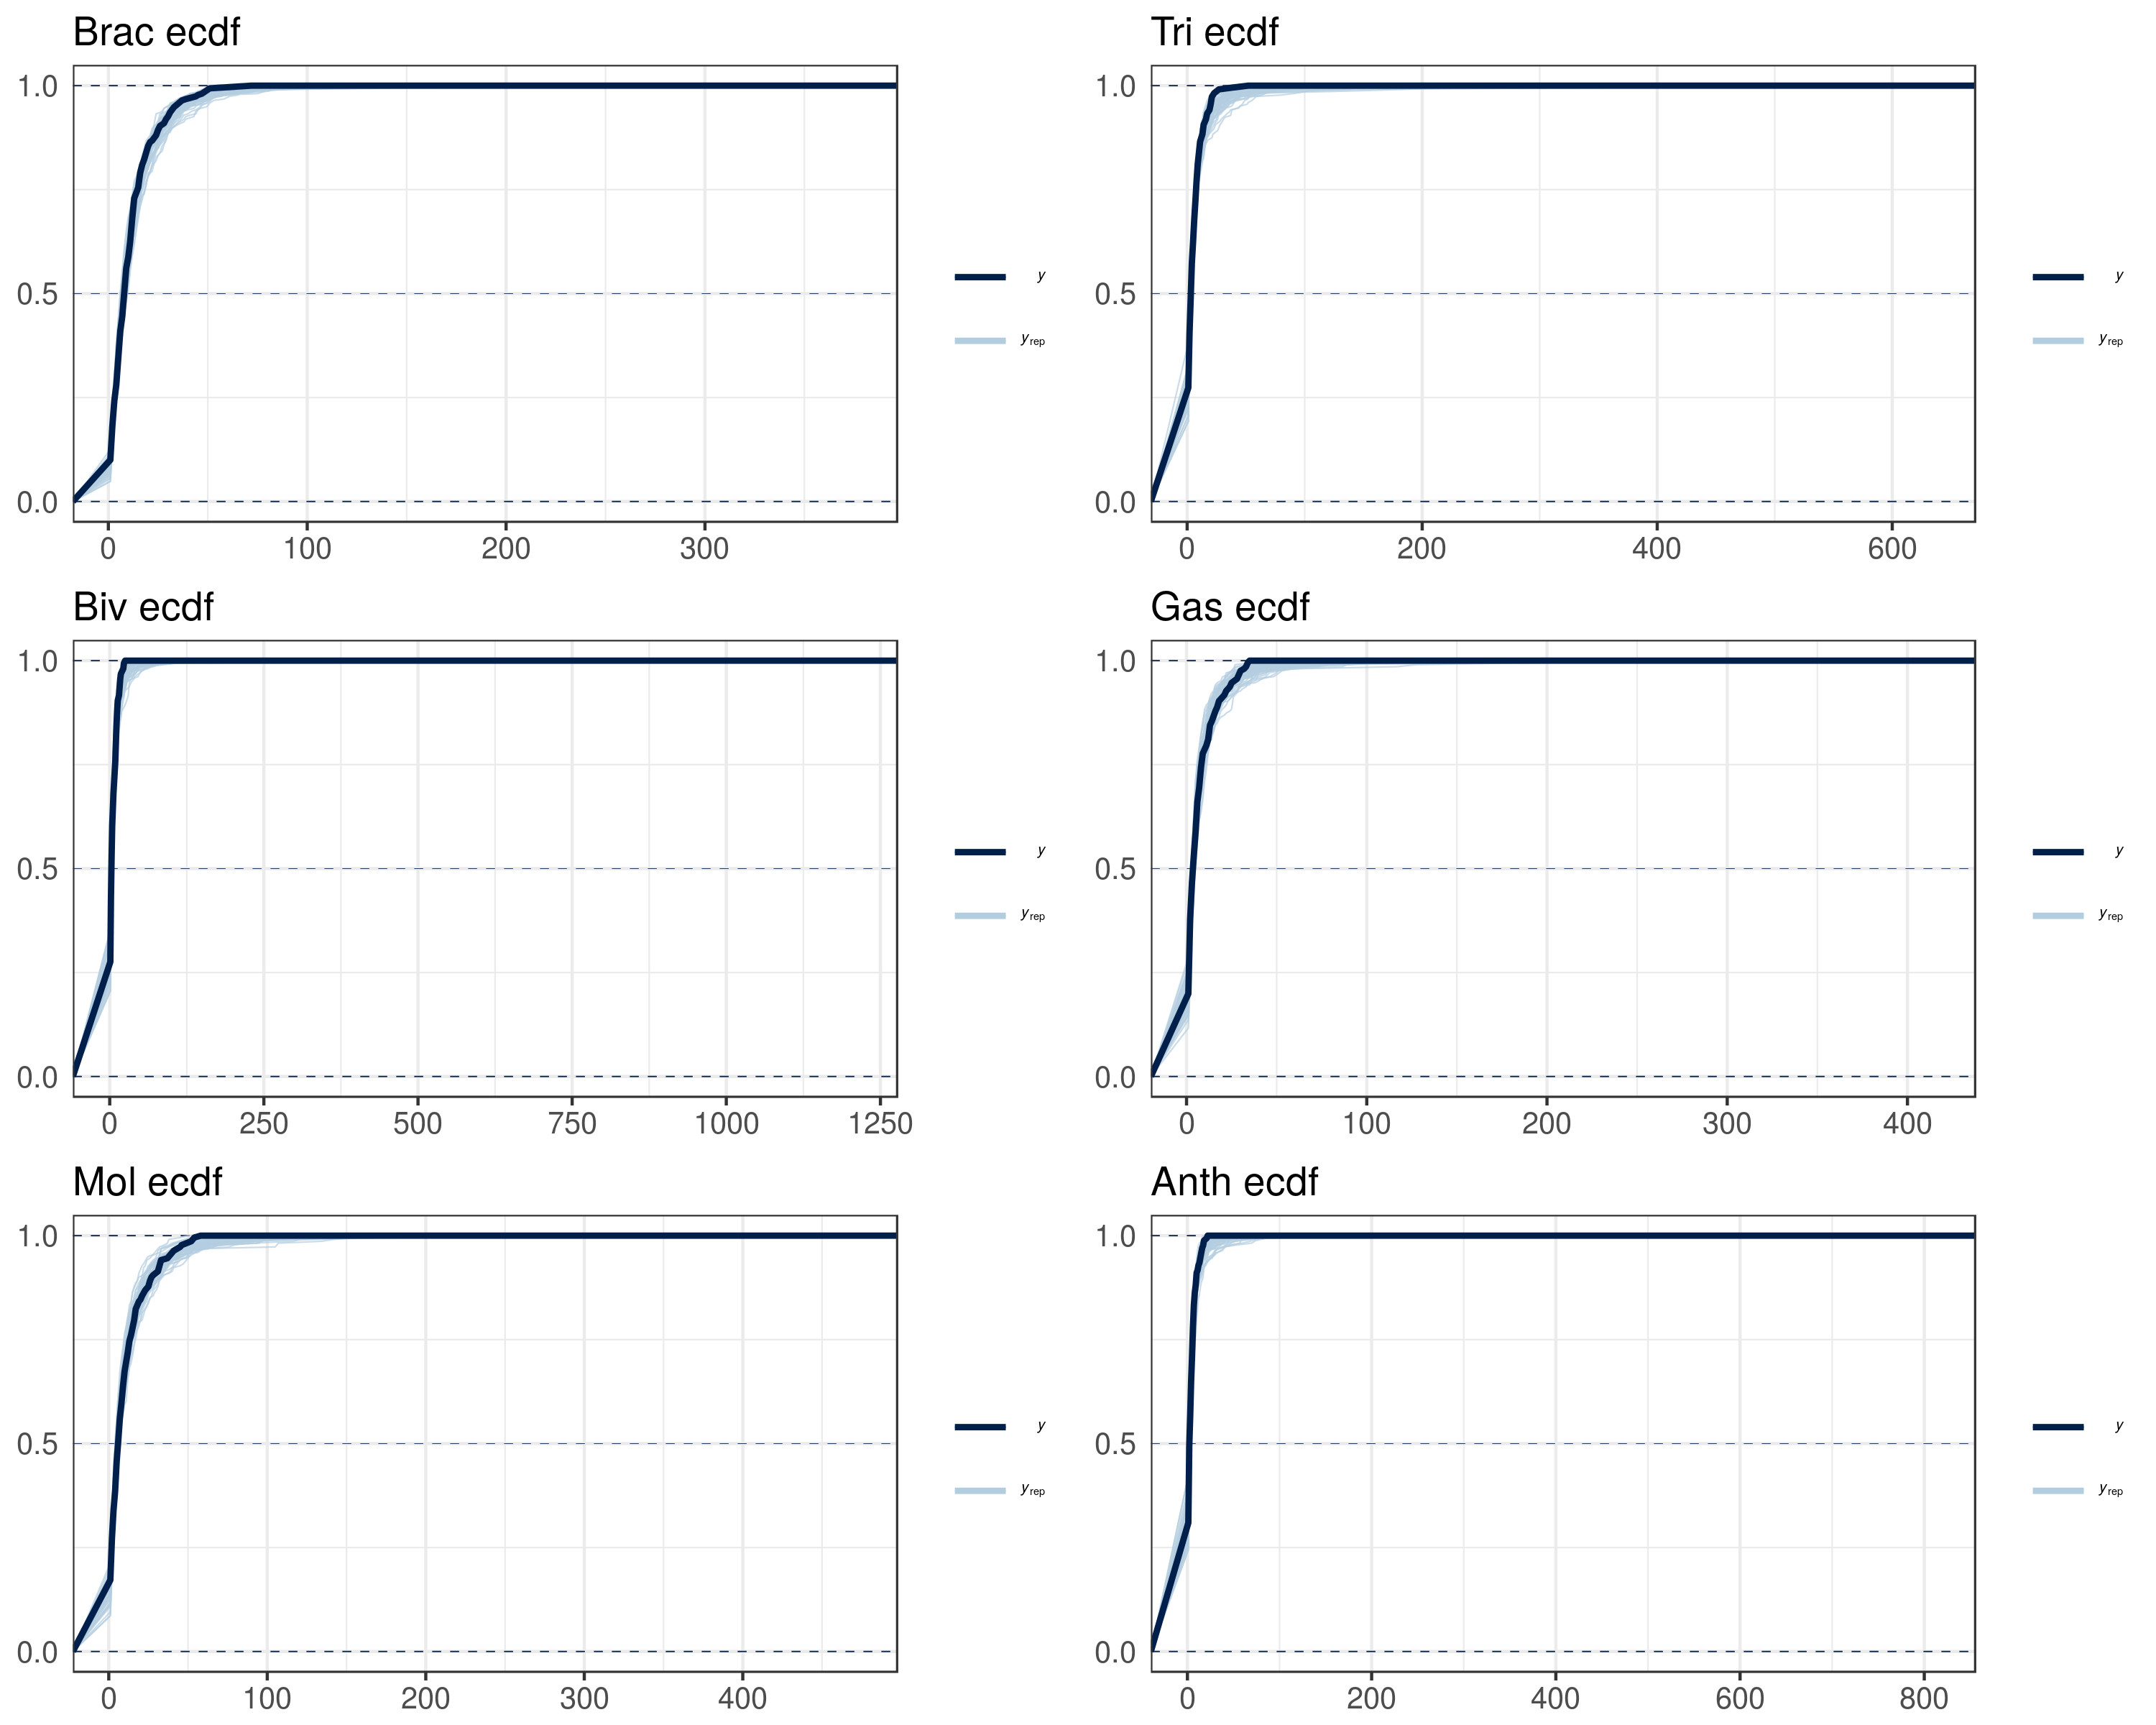
\includegraphics[width=\textwidth,height=0.5\textheight,keepaspectratio=true]{figure/ppc_ecdf}
  \caption{Posterior predictive results comparing the empirical cummulative distribution function (ecdf) of a geological unit for each of the studied taxonomic groups to a distribution of 1000 estimates from datasets simulated from the posterior predictive distribution of our models. Model adequacy is determined by how similar the posterior predictive distribution is to the observed value. In all cases, our models appear able to almost reproduce to observed ecdf-s.}
  \label{fig:ppc_ecdf}
\end{figure}






\subsection{Estimated versus observed unit diversity}
% what is the point of this section?
%   graph unit diversity by time bin
%   compare to estimate from model
%   this is like the ppc for group mean, but inside-out
%   if model has poor estimates for time bin
%     that bin is not like what we would expect based on our model
%   if we have good estimates for all bins
%     then we need to look at covariates to see if there are any switch patterns


% time series graph
% what does this graph represent?
%   geological unit diversity counts at time bins
%   comparison to posterior predictive mean est with 80CI
\begin{figure}[ht]
  \centering
  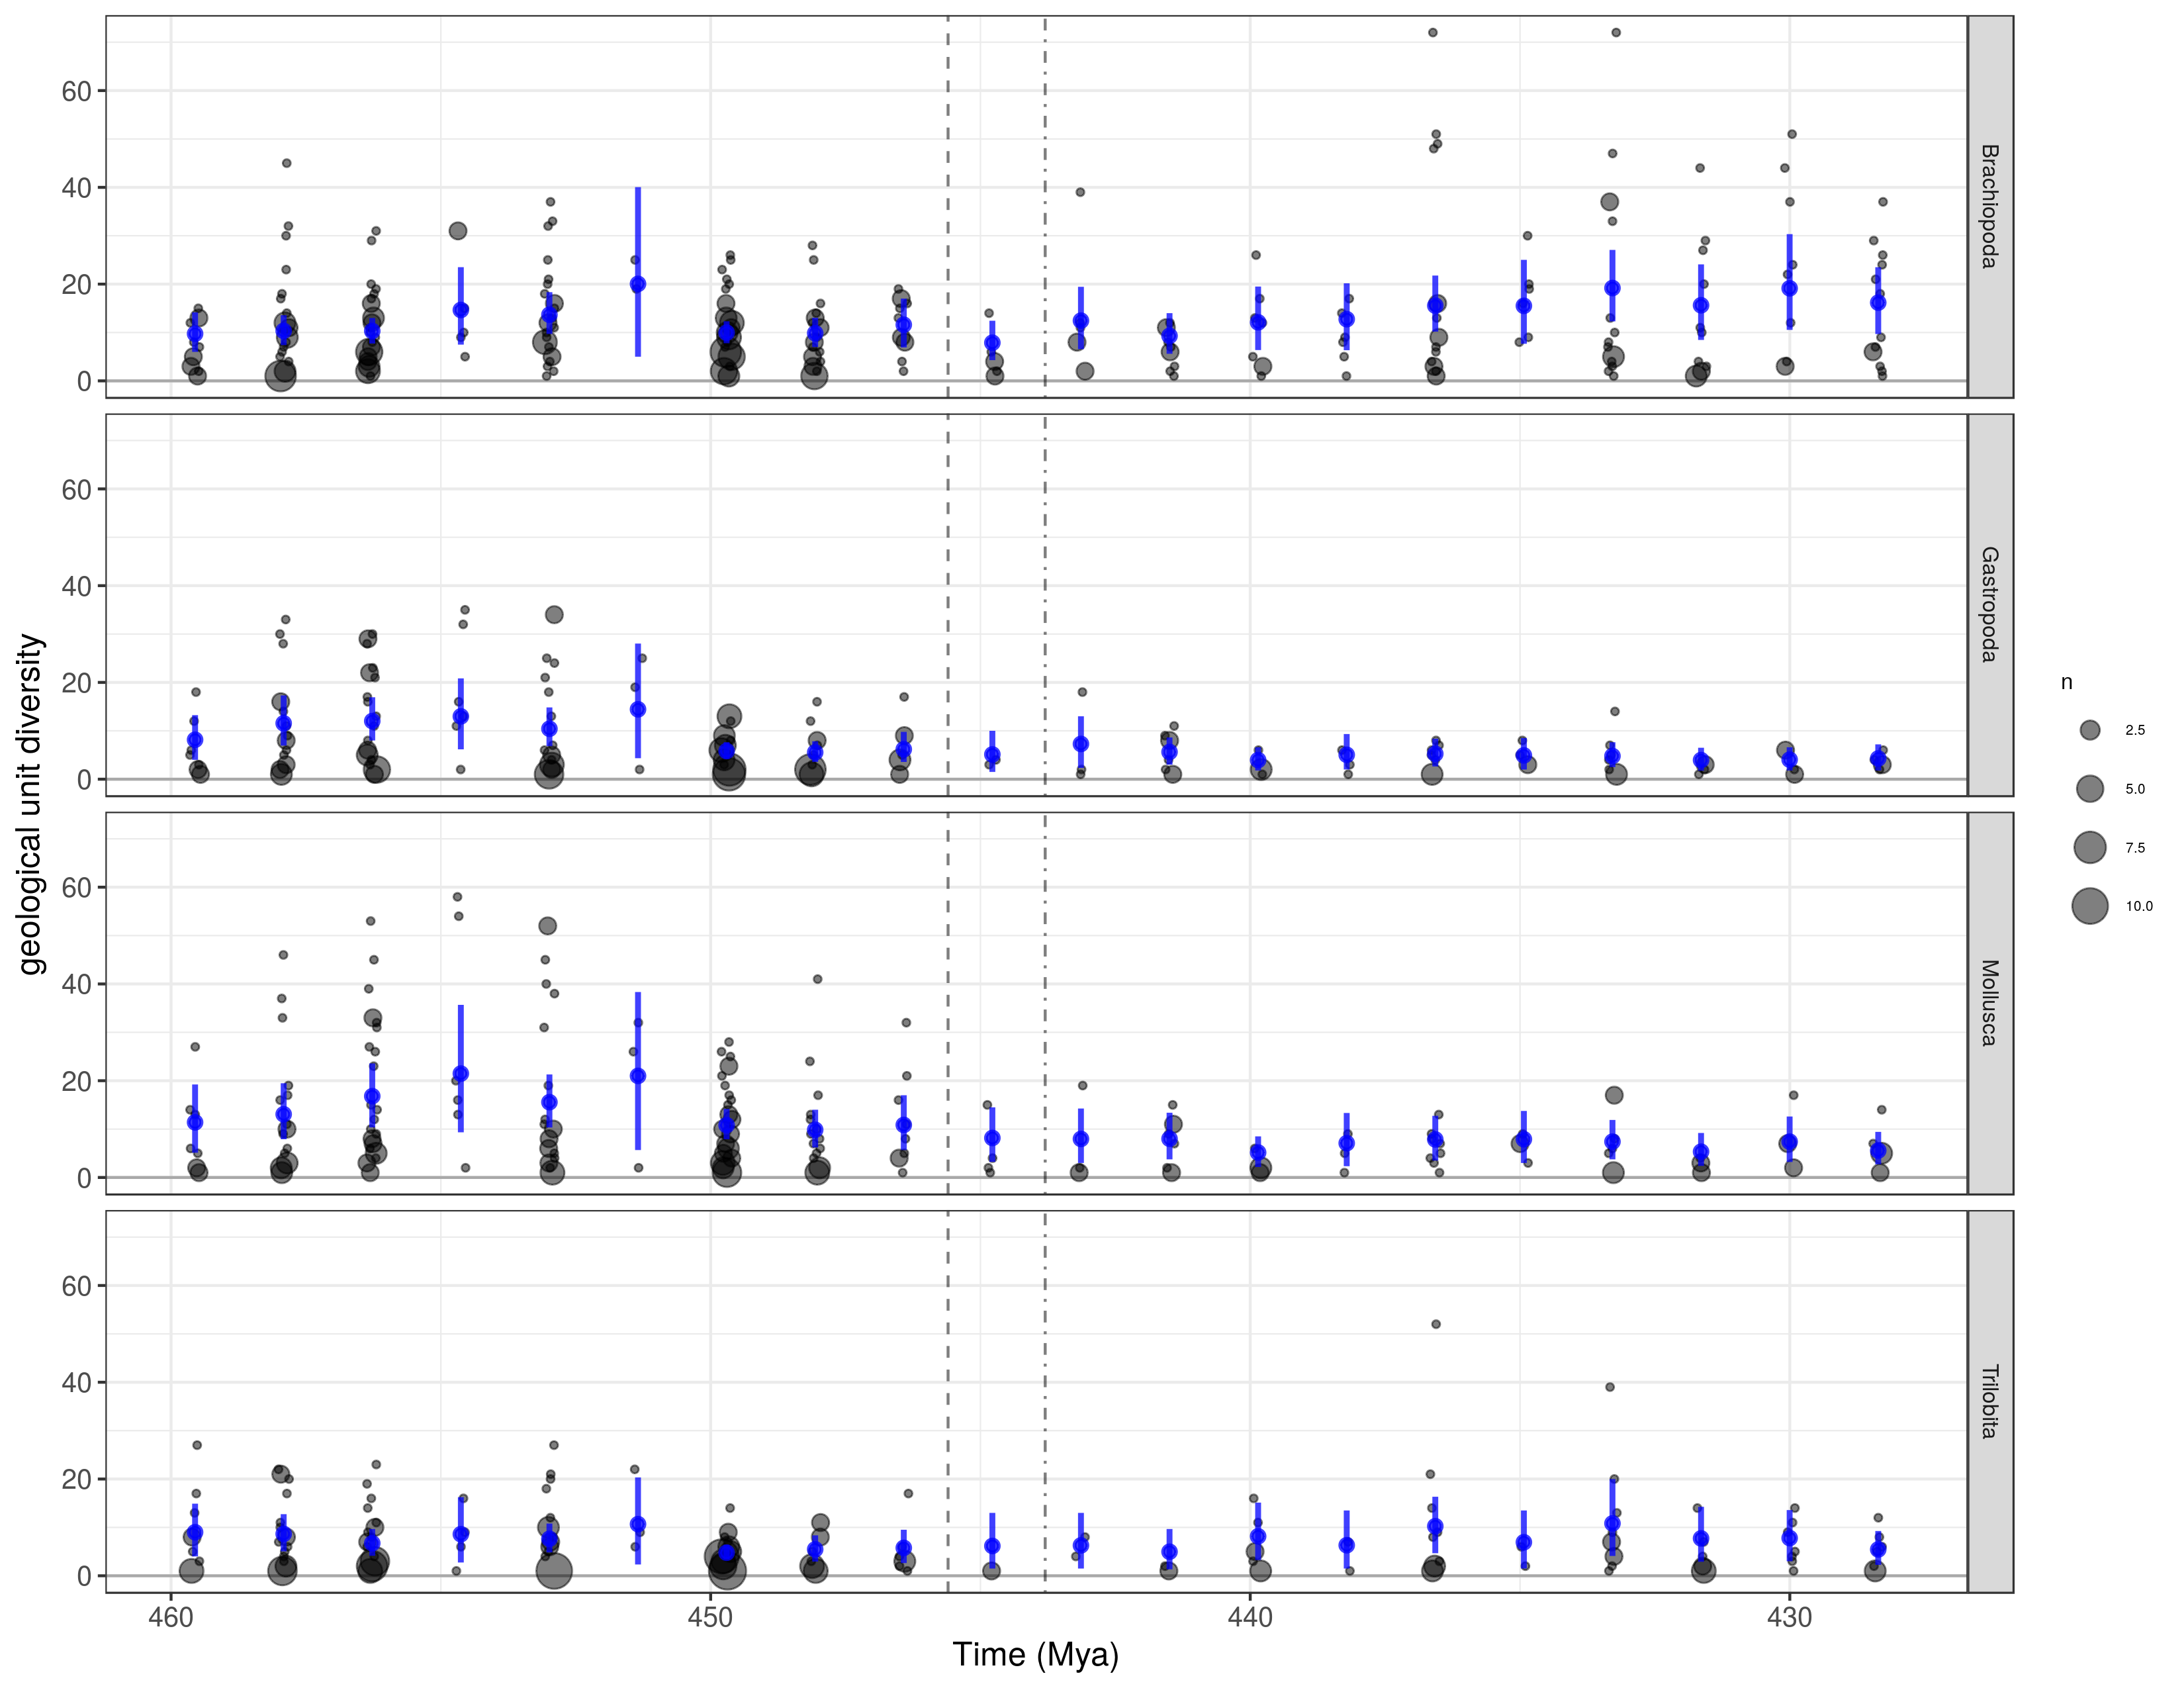
\includegraphics[width=\textwidth,height=0.5\textheight,keepaspectratio=true]{figure/unitdiv_time}
  \caption{Geological unit diversity though time and the expected diversity (with 80\% credible interval) as estimated from our models. Unit diversity is presented as partially transparent points and our jittered in the y-axis to improve readability. Point size is proportional to the number of units in that interval that have identical unit diversity. The dashed grey line corresponds to the onset of the Hirnantian geological stage, while the dashed-dotted grey line corresponds to the end of the Ordovician epoch and the start of the Silurian epoch.}
  \label{fig:time_div}
\end{figure}

\begin{figure}[ht]
  \centering
  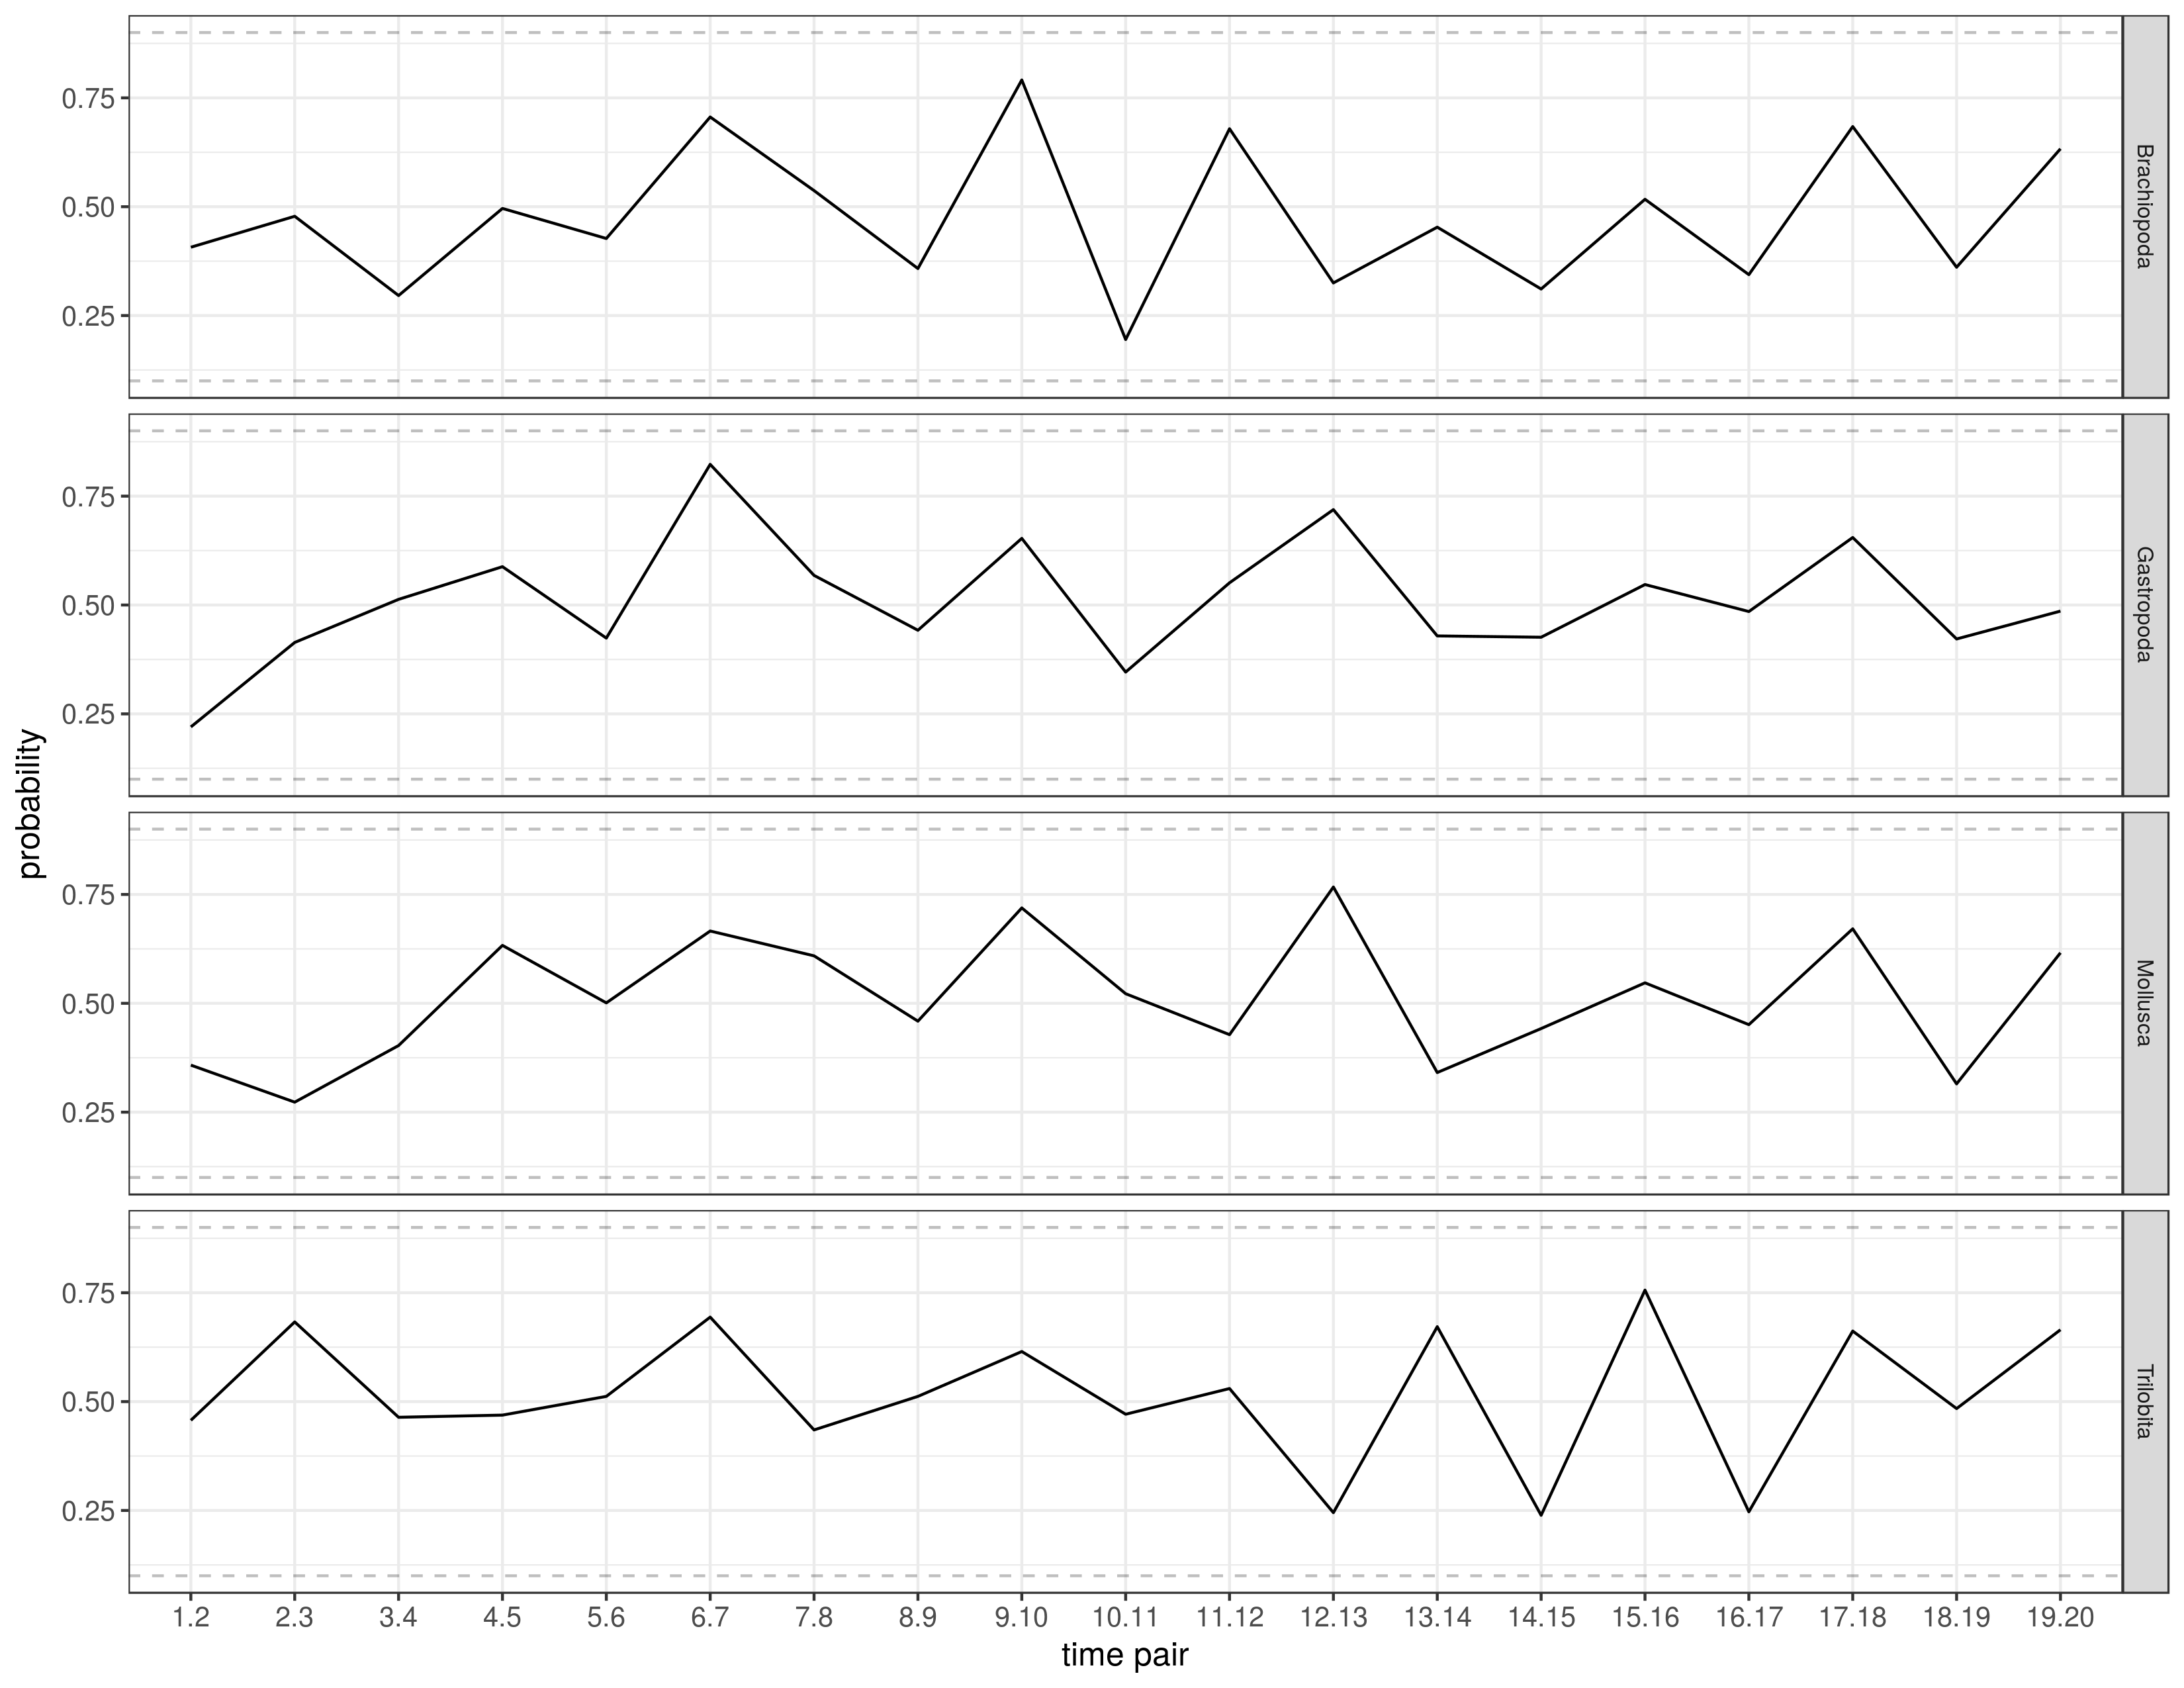
\includegraphics[width=\textwidth,height=0.5\textheight,keepaspectratio=true]{figure/unitdiv_diff}
  \caption{Probability that our estimate of mean unit diversity at time \(t\) is greater than the estimate at time \(t + 1\). The dashed grey horizontal lines correspond to probability of 0.8 and 0.2; these are the thresholds we chose as indicating if a pair-wise difference is potentially larger (or smaller) than no-difference (\(P = 0.5\)), and worthy of further inspection.}
  \label{fig:diff_div}
\end{figure}

% covariance of effect change?



\subsection{Effects of geological covariates on estimated diversity}
% what is the point of this section?
%   we've estimated the effect of multiple covariates
%   these estimates are allowed to vary through time
%     temporal structure is taken into account
%   what is the general relationship? what happens during hirnantian?
%     if all units have the same relationship
%       and all good bin estimates
%         there is no change in unit diversity though time
%         there is no change in geol properties that affect unit diversity
%       and some bad bin estimates
%         our model can not explain these bins; something is going on here
%     if some units have diff relationships (sign change, effect loss)
%       and all good bin estimates
%         we capture the changing relationship between preservational context and observed diversity
%       and some bad bin estimates
%         our model can not explain these bins; something is going on here


% time series graph
% what does this graph represent?
%   effect of covariate on expected count over time
%   violin shows full posterior estimate
%   pointrange shows mean with 80CI
\begin{figure}[ht]
  \centering
  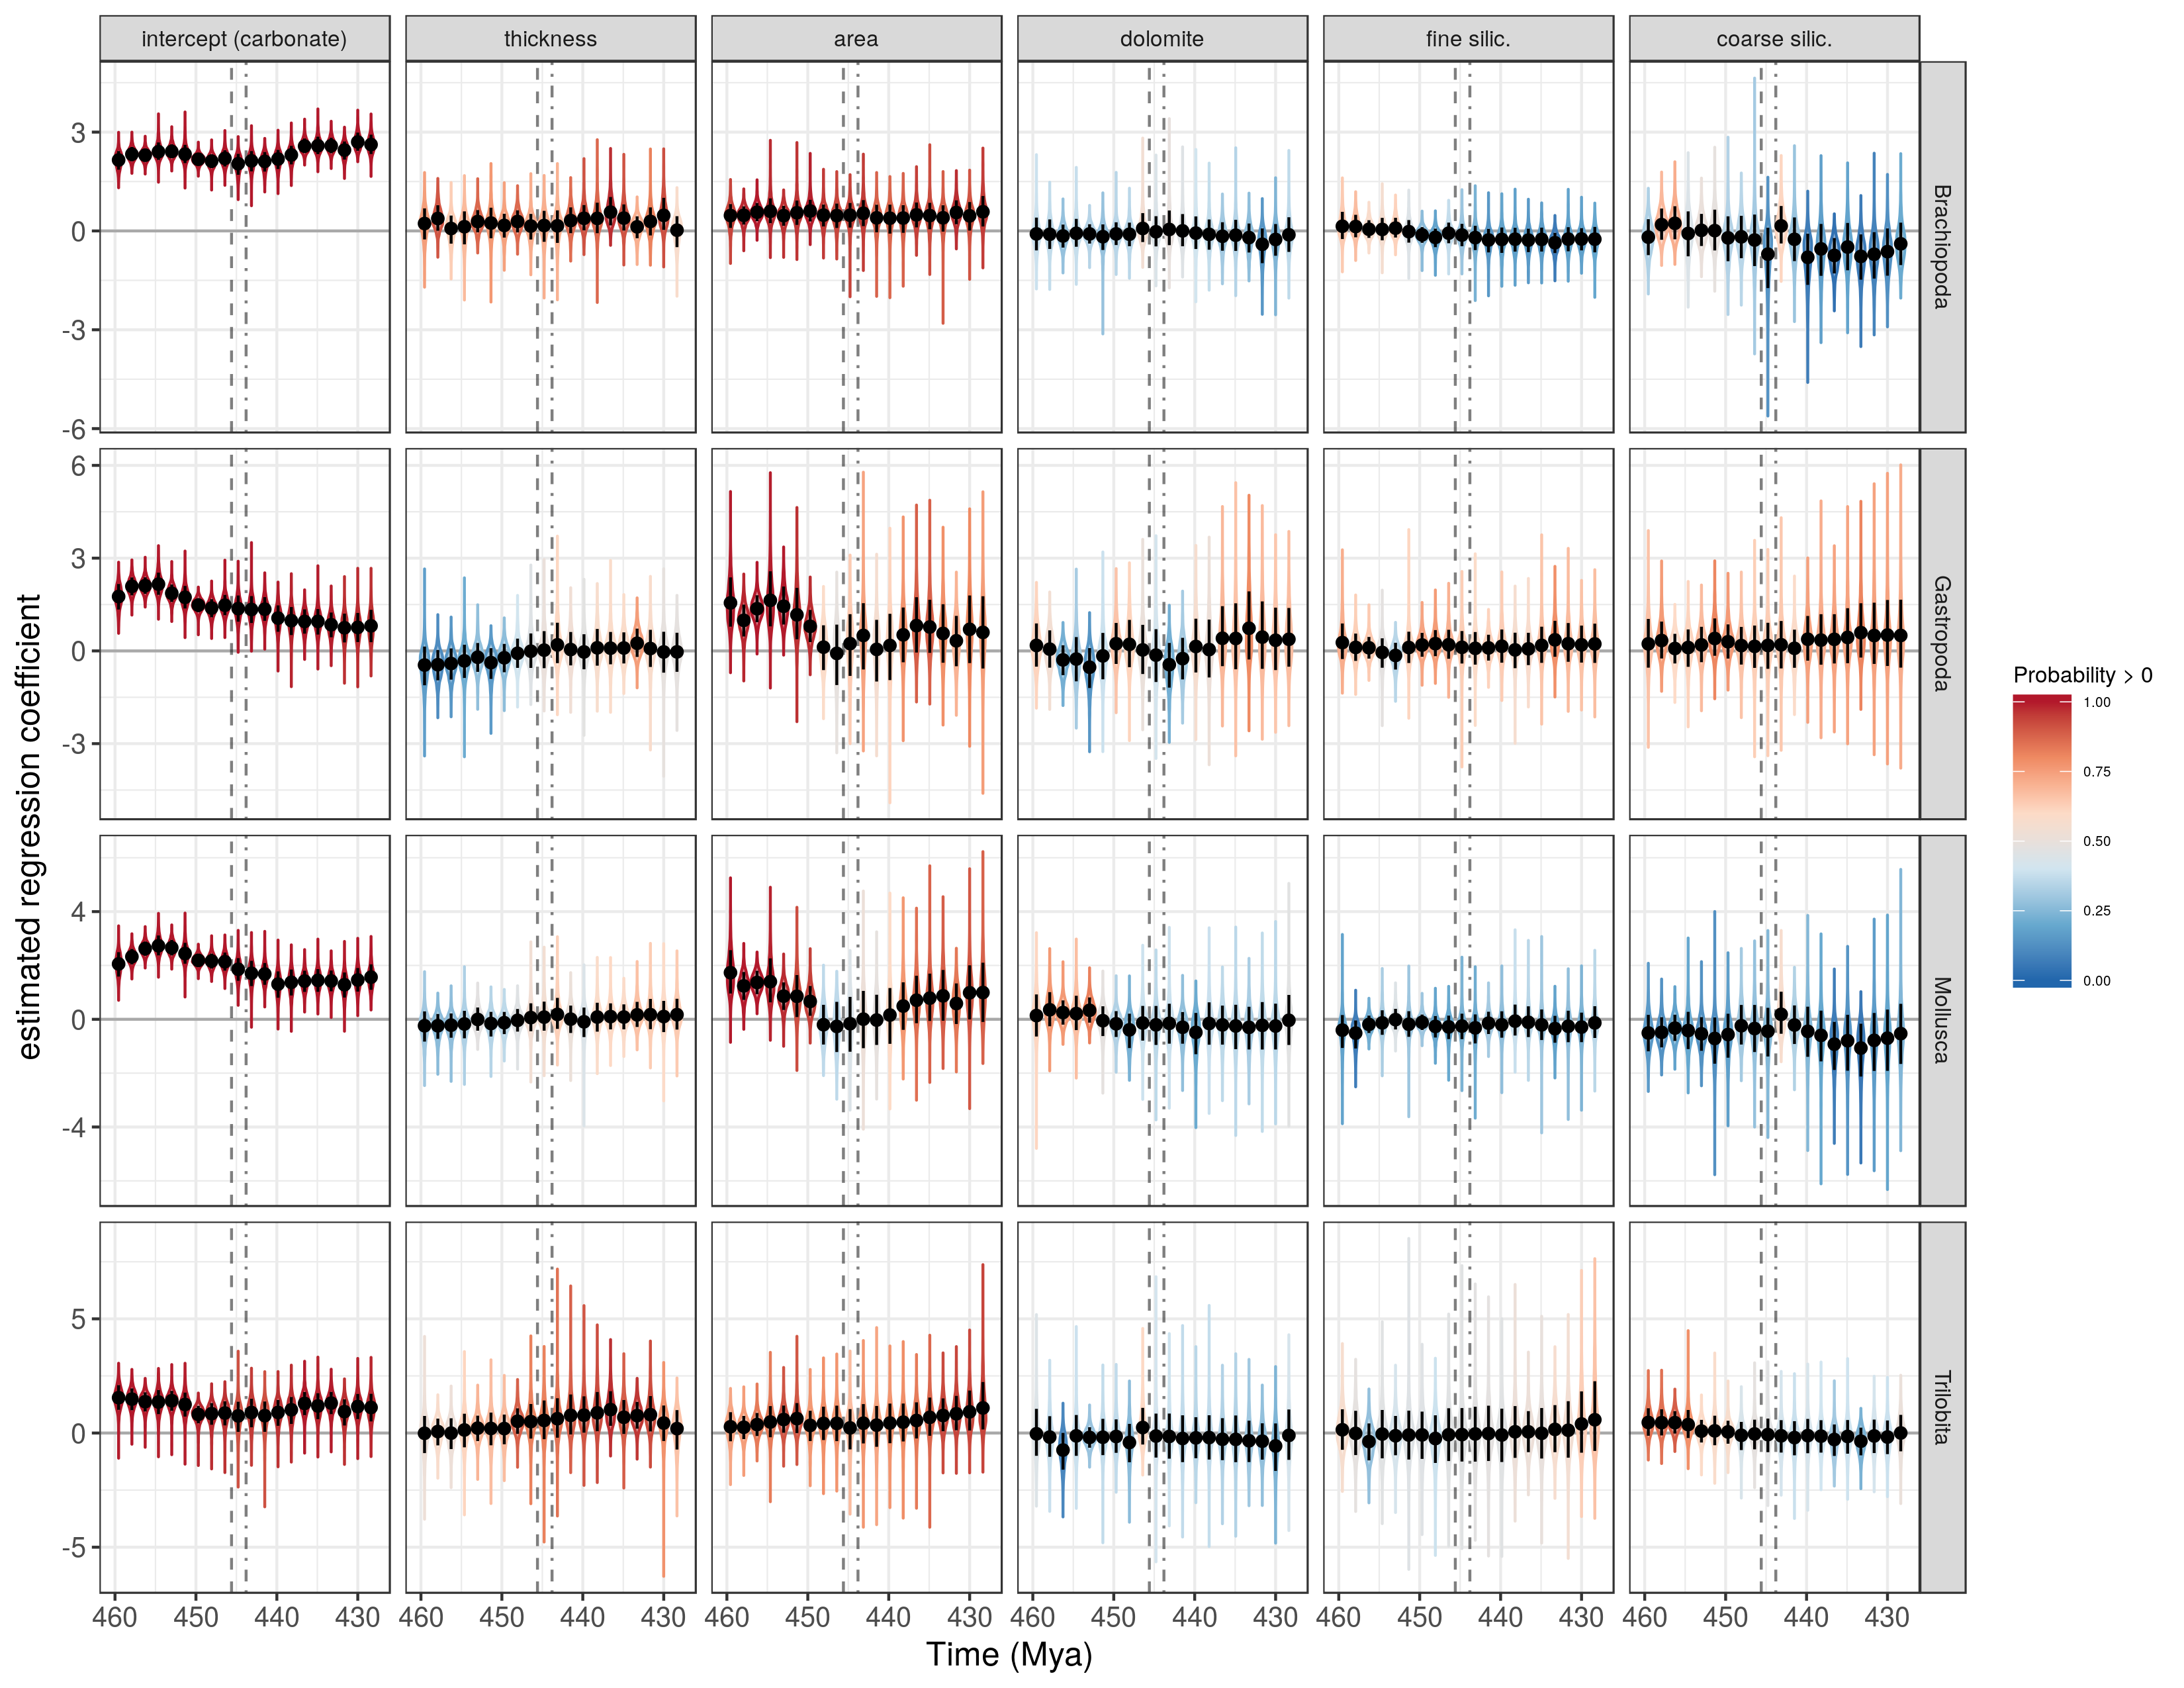
\includegraphics[width=\textwidth,height=0.5\textheight,keepaspectratio=true]{figure/cov_time}
  \caption{Estimates of all estimated covariate effect time series for each of the analyzed taxonomic groups, including intercept estimates. Points represent mean estimate along with a 80\% credible interval. The black horizontal line corresponds to no effect. Points are plotted at the mid-point of the discrete time interval.}
  \label{fig:time_cov}
\end{figure}

\begin{figure}[ht]
  \centering
  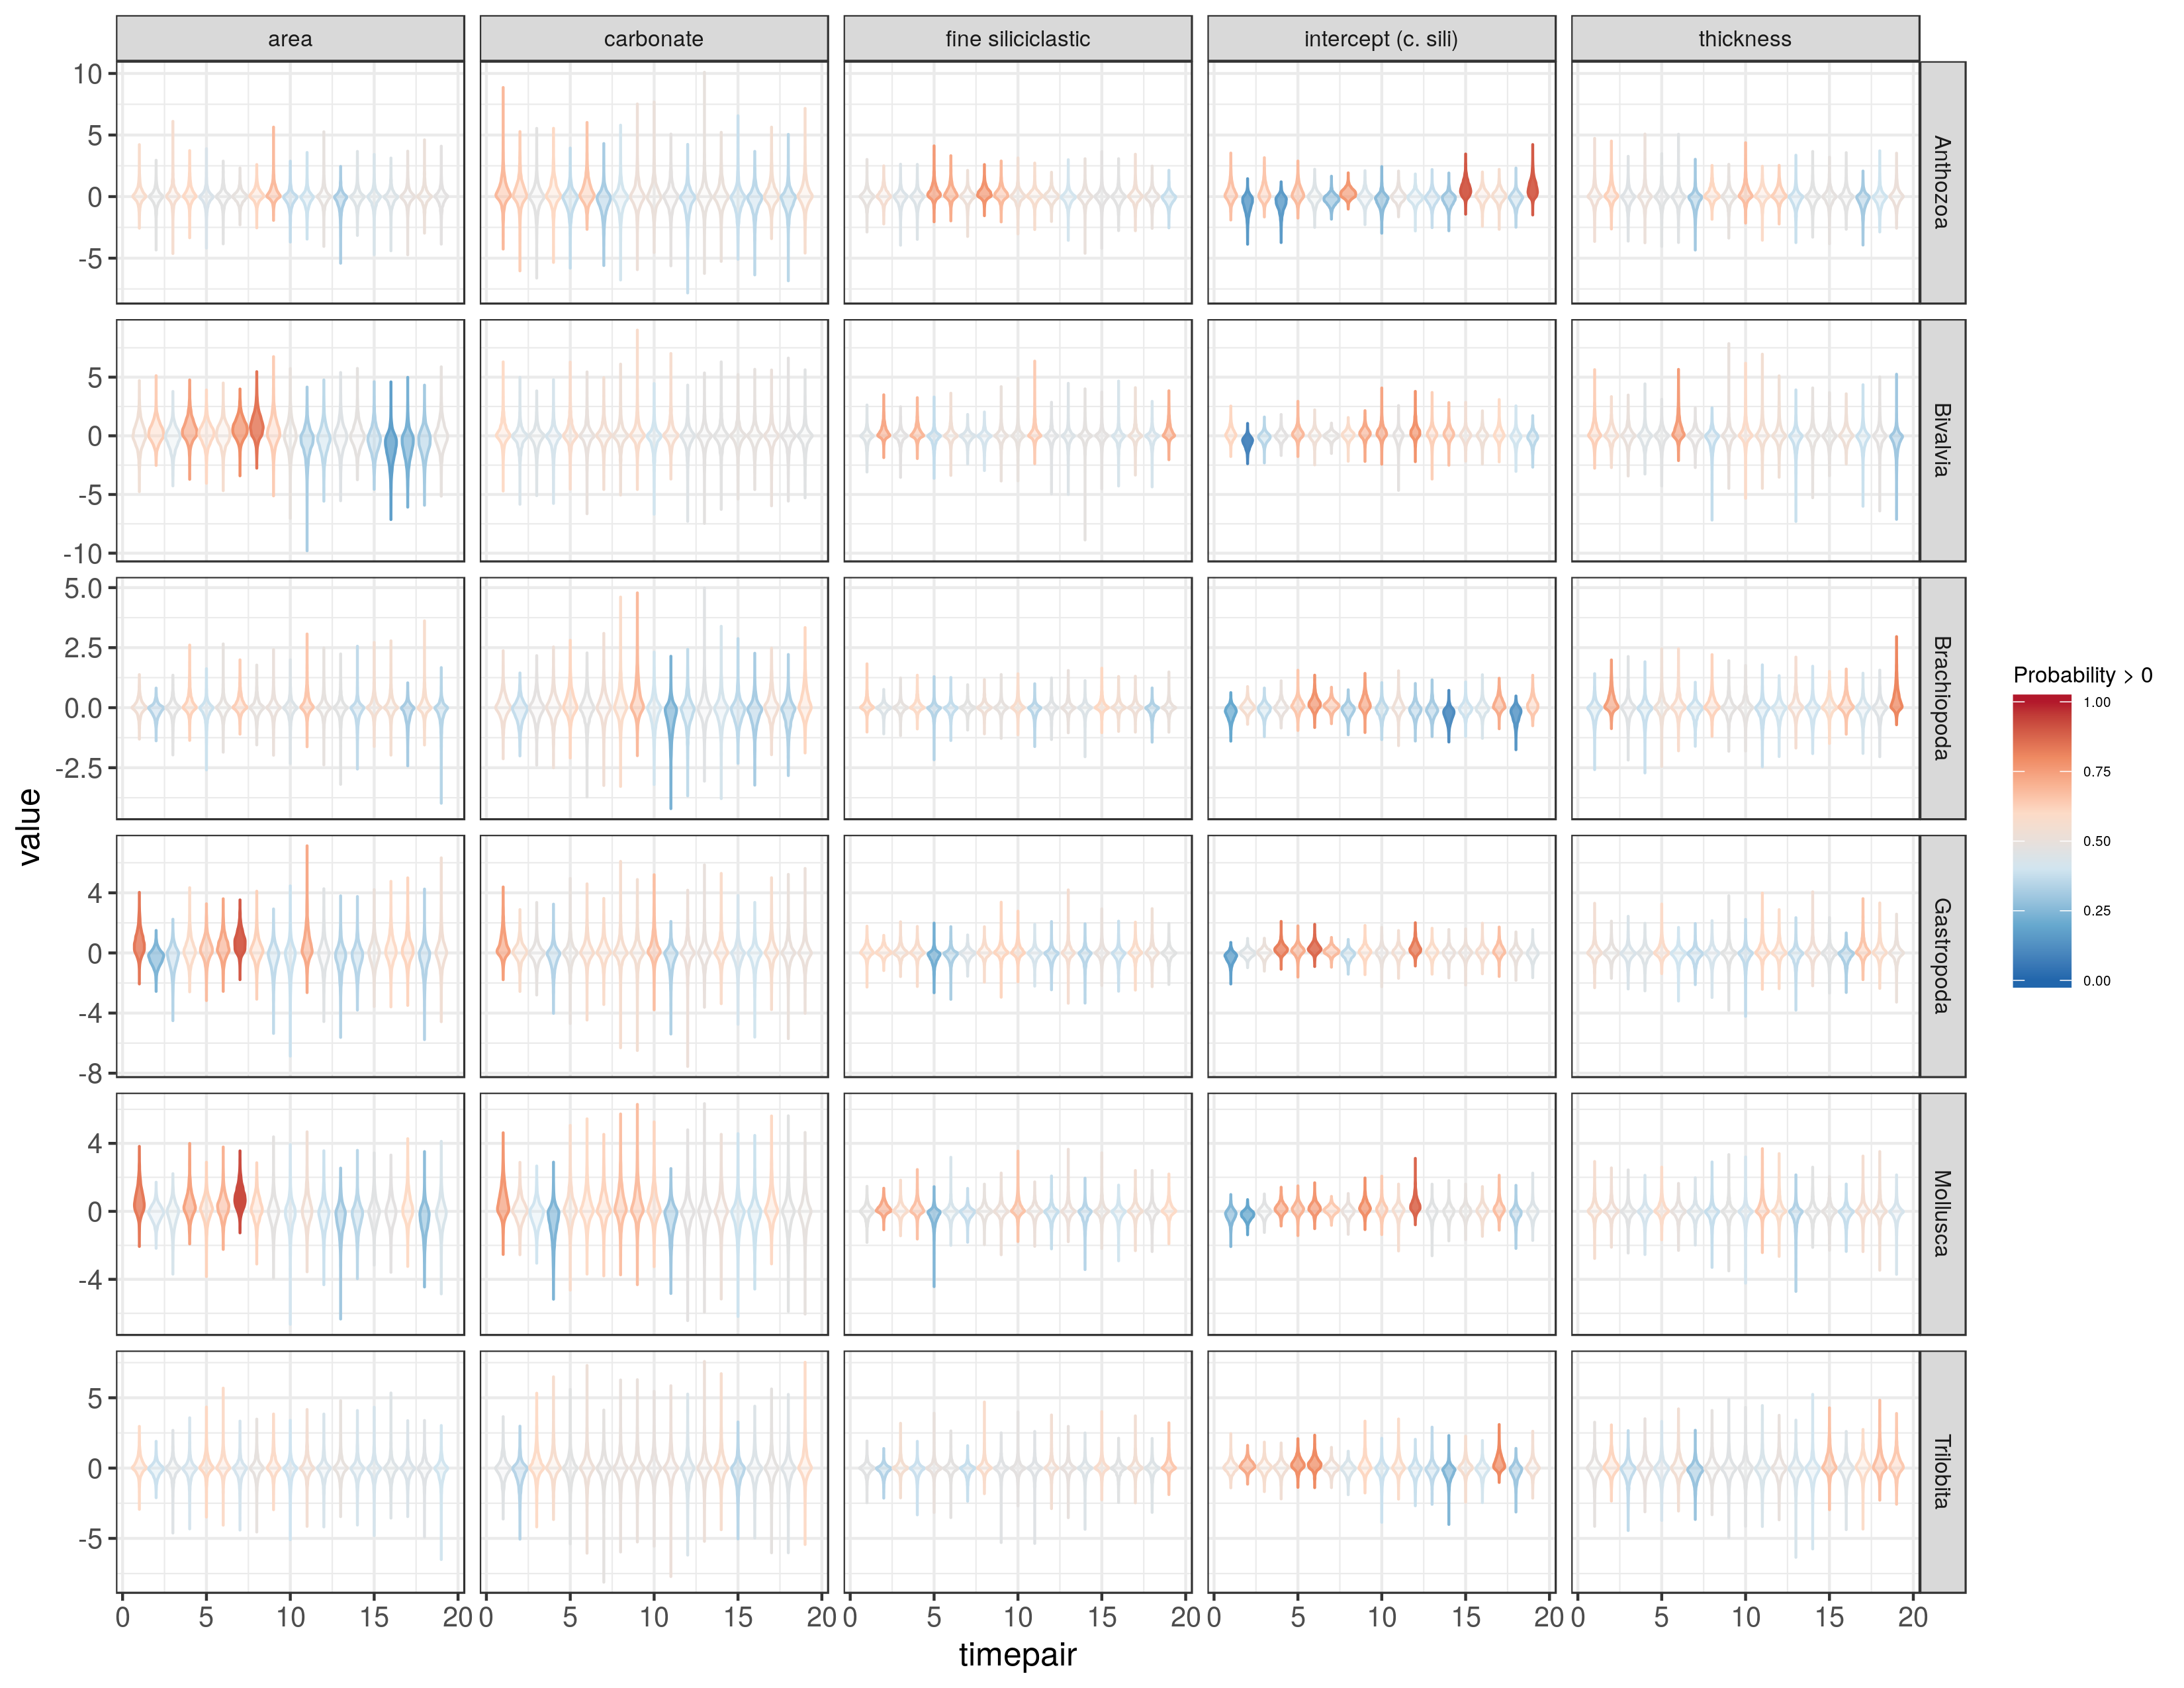
\includegraphics[width=\textwidth,height=0.5\textheight,keepaspectratio=true]{figure/cov_diff}
  \caption{Probability that a parameter estimate at time \(t\) is greater than the estimate at time \(t + 1\). The dashed grey horizontal lines correspond to probability of 0.8 and 0.2; these are the thresholds we chose as indicating if a pair-wise difference is potentially larger (or smaller) than no-difference (\(P = 0.5\)), and worthy of further inspection.}
  \label{fig:diff_cov}
\end{figure}

% covariance of effect change?
%   are effects correlated in their changes through time?







\begin{figure}[ht]
  \centering
  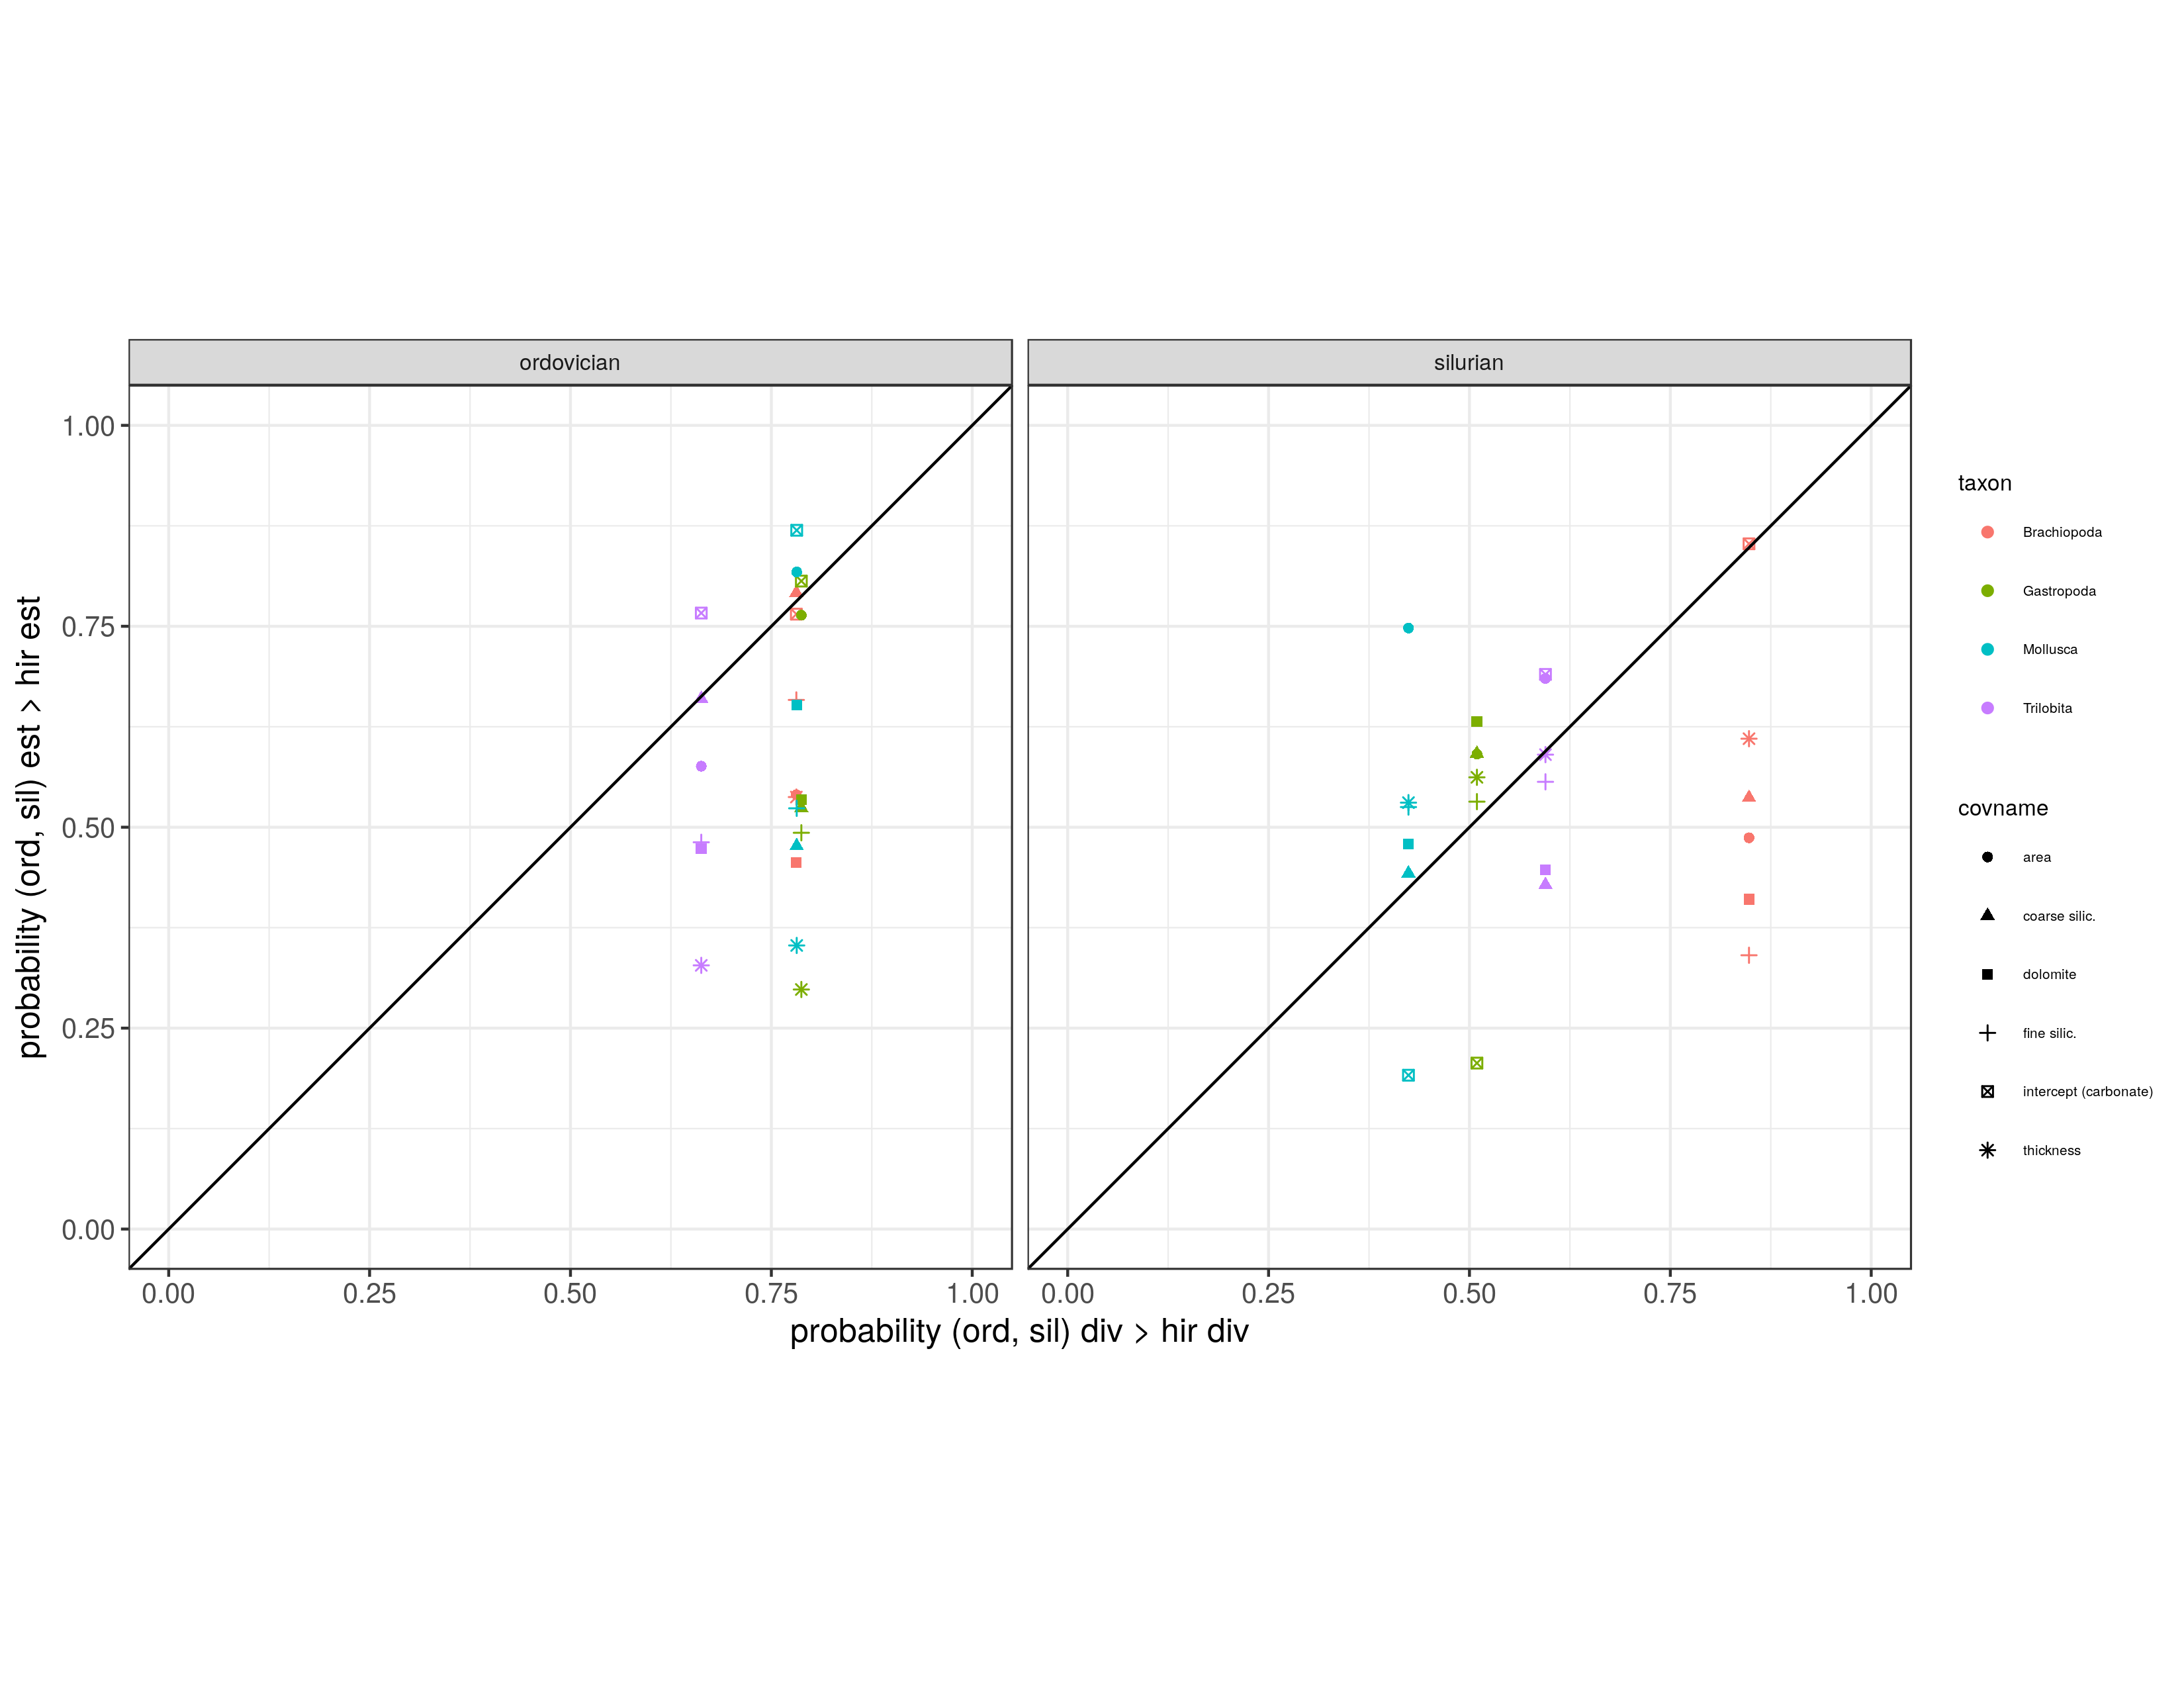
\includegraphics[width=\textwidth,height=0.5\textheight,keepaspectratio=true]{figure/compare_pval}
  \caption{Scatterplot of the estimated probability that geological unit diversity is lower during the Hirnantian than either the Ordovician (left facet) or the Silurian (right facet) vs the estimated probability that a covariate estimate is lower during the Hirnantian than either the Ordovician or the Silurian. For each of the taxonomic groups there is only one estimate for the probability of difference in diversity, but there are six probability estimates for each of the covariate effect parameters. }
  \label{fig:<+label+>}
\end{figure}<++>


\end{document}
